\documentclass{article}

\usepackage{fancyhdr}
\usepackage{extramarks}
\usepackage{amsmath,mathrsfs,amssymb}
\usepackage{amsthm}
\usepackage{amsfonts}
\usepackage{tikz}
\usepackage[plain]{algorithm}
\usepackage{algpseudocode}
\usepackage[]{mcode}
\usepackage{graphicx}
\usepackage{pgfplots}
\usepackage{xfrac}

\usetikzlibrary{automata,positioning}

%
% Basic Document Settings
%

\topmargin=-0.45in
\evensidemargin=0in
\oddsidemargin=0in
\textwidth=6.5in
\textheight=9.0in
\headsep=0.25in

\linespread{1.1}

\pagestyle{fancy}
\lhead{\hmwkAuthorName}
\chead{\hmwkClass\ (\hmwkClassInstructor\ \hmwkClassTime): \hmwkTitle}
\rhead{\firstxmark}
\lfoot{\lastxmark}
\cfoot{\thepage}

\renewcommand\headrulewidth{0.4pt}
\renewcommand\footrulewidth{0.4pt}

\setlength\parindent{0pt}

%
% Create Problem Sections
%

\newcommand{\enterProblemHeader}[1]{
    \nobreak\extramarks{}{Problem \arabic{#1} continued on next page\ldots}\nobreak{}
    \nobreak\extramarks{Problem \arabic{#1} (continued)}{Problem \arabic{#1} continued on next page\ldots}\nobreak{}
}

\newcommand{\exitProblemHeader}[1]{
    \nobreak\extramarks{Problem \arabic{#1} (continued)}{Problem \arabic{#1} continued on next page\ldots}\nobreak{}
    \stepcounter{#1}
    \nobreak\extramarks{Problem \arabic{#1}}{}\nobreak{}
}

\setcounter{secnumdepth}{0}
\newcounter{partCounter}
\newcounter{homeworkProblemCounter}
\setcounter{homeworkProblemCounter}{1}
\nobreak\extramarks{Problem \arabic{homeworkProblemCounter}}{}\nobreak{}

%
% Homework Problem Environment
%
% This environment takes an optional argument. When given, it will adjust the
% problem counter. This is useful for when the problems given for your
% assignment aren't sequential. See the last 3 problems of this template for an
% example.
%
\newenvironment{homeworkProblem}[1][-1]{
    \ifnum#1>0
        \setcounter{homeworkProblemCounter}{#1}
    \fi
    \section{Problem \arabic{homeworkProblemCounter}}
    \setcounter{partCounter}{1}
    \enterProblemHeader{homeworkProblemCounter}
}{
    \exitProblemHeader{homeworkProblemCounter}
}

%
% Homework Details
%   - Title
%   - Due date
%   - Class
%   - Section/Time
%   - Instructor
%   - Author
%

\newcommand{\hmwkTitle}{Tutorial\ 2}
\newcommand{\hmwkDueDate}{April 25, 2016}
\newcommand{\hmwkClass}{Systems Modelling and Control}
\newcommand{\hmwkClassTime}{}
\newcommand{\hmwkClassInstructor}{Damien Hill}
\newcommand{\hmwkAuthorName}{S.Reynolds (262538)}

%
% Title Page
%

\title{
    \vspace{2in}
    \textmd{\textbf{\hmwkClass:\ \hmwkTitle}}\\
    \normalsize\vspace{0.1in}\small{Due\ on\ \hmwkDueDate\ at 3:10pm}\\
    \vspace{0.1in}\large{\textit{\hmwkClassInstructor\ \hmwkClassTime}}
    \vspace{3in}
}

\author{\textbf{\hmwkAuthorName}}
\date{}

\renewcommand{\part}[1]{\textbf{\large Part \Alph{partCounter}}\stepcounter{partCounter}\\}

%
% Various Helper Commands
%

% Useful for algorithms
\newcommand{\alg}[1]{\textsc{\bfseries \footnotesize #1}}

% For derivatives
\newcommand{\deriv}[1]{\frac{\mathrm{d}}{\mathrm{d}x} (#1)}

% For partial derivatives
\newcommand{\pderiv}[2]{\frac{\partial}{\partial #1} (#2)}

% Integral dx
\newcommand{\dx}{\mathrm{d}x}

% Alias for the Solution section header
\newcommand{\solution}{\textbf{\large Solution}}

% Probability commands: Expectation, Variance, Covariance, Bias
\newcommand{\E}{\mathrm{E}}
\newcommand{\Var}{\mathrm{Var}}
\newcommand{\Cov}{\mathrm{Cov}}
\newcommand{\Bias}{\mathrm{Bias}}

\DeclareMathOperator{\sinc}{sinc}

\begin{document}

\maketitle

\pagebreak

%%%%%%%%%%%%%%%%%%%%%%%%%%%%%%%%%%%%%%%%%%%%%%%%%%%%%%%%%%%%%%%%%%%%%%%%%%%%%%%%%%%%%%%%%%%%%%%%%%%%%%%%%%%%%%%%%%%%%%
% Question 1
%%%%%%%%%%%%%%%%%%%%%%%%%%%%%%%%%%%%%%%%%%%%%%%%%%%%%%%%%%%%%%%%%%%%%%%%%%%%%%%%%%%%%%%%%%%%%%%%%%%%%%%%%%%%%%%%%%%%%% 

\begin{homeworkProblem}
    \textbf{Fourier Transforms}\\
    
    A periodic signal, $x(t)$, with period $T$ has Fourier coefficients $c^{x}_{k}$ such that:
    
    \begin{align*}
	    x(t) = \sum_{k = -\infty}^{\infty}c^{x}_{k}e^{jk \omega_{0} t}, \quad \omega_{0} = \frac{2 \pi}{T}, \quad -\infty<t<\infty
    \end{align*}
    
    \vspace{5mm}
    
    \textsc{Question a}\\
    
    If $v(t) = x(t - 1)$, then:
    
    \begin{align*}
	    v(t) 	&= \sum_{k = -\infty}^{\infty} c^{x}_{k} e^{jk \omega_{0} (t-1)}\\
			    &= \sum_{k = -\infty}^{\infty} c^{x}_{k} e^{jk \omega_{0}t - jk \omega_{0}}\\
			    &= \sum_{k = -\infty}^{\infty} c^{x}_{k} e^{jk \omega_{0}t} e^{-jk \omega_{0}}\\
			    &= \sum_{k = -\infty}^{\infty} e^{-jk \omega_{0}} c^{x}_{k} e^{jk \omega_{0}t}\\
    \end{align*}
    
    Hence, we find that $c^{v}_{k} = e^{-jk \omega_{0}} c^{x}_{k}$.\\
    
    \vspace{5mm}
    
    \textsc{Question b}\\
    
    If $v(t) = \frac{dx(t)}{dt}$, then:
    
    \begin{align*}
	    v(t)	&= \frac{d}{dt} \bigg( \sum_{k = -\infty}^{\infty} c^{x}_{k} e^{jk \omega_{0}t} \bigg)
    \end{align*}
    
    We note at this point that generally it is not appropriate to simply move a differential operator inside an infinite series, however, in this instance we will assume that the necessary conditions for performing this operation are satisfied. Hence, we get:
    
    \begin{align*}
	    v(t)	&= \sum_{k = -\infty}^{\infty} c^{x}_{k} \frac{d}{dt}(e^{jk \omega_{0}t})\\
			    &= \sum_{k = -\infty}^{\infty} c^{x}_{k} jk \omega_{0} (e^{jk \omega_{0}t})\\
			    &= \sum_{k = -\infty}^{\infty} jk \omega_{0} c^{x}_{k} e^{jk \omega_{0}t}
    \end{align*}
    
    Hence, we find that $c^{v}_{k} = jk \omega_{0} c^{x}_{k}$.\\
    
    \vspace{5mm}
    
    \textsc{Question c}\\
    
    If $v(t) = x(t)e^{j \omega_0 t}$, then:
    
    \begin{align*}
	    v(t)	&= e^{j \omega_0 t} \sum_{k = -\infty}^{\infty} c^{x}_{k} e^{jk \omega_{0}t}\\
			    &= \sum_{k = -\infty}^{\infty} c^{x}_{k} e^{j \omega_0 t} e^{jk \omega_{0}t}\\
			    &= \sum_{k = -\infty}^{\infty} c^{x}_{k} e^{j \omega_{0}t(k+1)}\\
    \end{align*}
    
    Since the sum is over an infinite series, we can change $c^{k}_{x}$ to $c^{k-1}_{x}$ and change $(k+1)$ to simply $k$ and we get the following:
    
    \begin{align*}
	    v(t)	&= \sum_{k = -\infty}^{\infty} c^{x}_{k-1} e^{j \omega_{0}tk}
    \end{align*}
    
    Hence, we find that $c^{v}_{k} = c^{x}_{k-1}$.\\
    
    \vspace{5mm}
    
    \textsc{Question d}\\
    
    If $v(t) = x(t)\cos(\frac{2 \pi}{T}t)$, then:
    
    \begin{align*}
	    v(t)	&= \cos(\frac{2 \pi}{T}t) \sum_{k = -\infty}^{\infty} c^{x}_{k} e^{jk \omega_{0}t}
    \end{align*}
    
    Since $\omega_0 = \frac{2 \pi}{T}$, we can re write this as:
    
    \begin{align*}
	     v(t)	&= cos(\omega_0 t) \sum_{k = -\infty}^{\infty} c^{x}_{k} e^{jk \omega_{0}t}\\
			    &= \sum_{k = -\infty}^{\infty} c^{x}_{k} e^{jk \omega_{0}t} cos(\omega_0 t)\\
			    &= \sum_{k = -\infty}^{\infty} c^{x}_{k} e^{jk \omega_{0}t} \frac{1}{2} (e^{j \omega_{0}t} + e^{-j \omega_{0}t})\\
			    &= \frac{1}{2} \sum_{k = -\infty}^{\infty} c^{x}_{k} e^{jk \omega_{0}t} (e^{j \omega_{0}t} + e^{-j \omega_{0}t})\\
			    &= \frac{1}{2} \sum_{k = -\infty}^{\infty} c^{x}_{k} e^{jk \omega_{0}t} e^{j \omega_{0}t} + c^{x}_{k} e^{jk \omega_{0}t} e^{-j \omega_{0}t}\\
			    &= \frac{1}{2} \sum_{k = -\infty}^{\infty} c^{x}_{k} e^{j \omega_{0}t(k+1)} + c^{x}_{k} e^{j \omega_{0}t(k-1)}
    \end{align*}
    
    Using the same idea that we used in question (c), we can re-write the series as follows:
    
    \begin{align*}
	    v(t)	 &= \frac{1}{2} \sum_{k = -\infty}^{\infty} c^{x}_{k-1} e^{j \omega_{0}tk} + c^{x}_{k+1} e^{j \omega_{0}tk}\\
				 &= \sum_{k = -\infty}^{\infty} \frac{1}{2} (c^{x}_{k-1} + c^{x}_{k+1}) e^{jk \omega_{0}t}\\
    \end{align*}
    
    Hence, we find that $c^{v}_{k} = \frac{1}{2} (c^{x}_{k-1} + c^{x}_{k+1})$.\\
    
    \vspace{5mm}
    
    
\end{homeworkProblem}

\pagebreak

%%%%%%%%%%%%%%%%%%%%%%%%%%%%%%%%%%%%%%%%%%%%%%%%%%%%%%%%%%%%%%%%%%%%%%%%%%%%%%%%%%%%%%%%%%%%%%%%%%%%%%%%%%%%%%%%%%%%%%
% Question 2
%%%%%%%%%%%%%%%%%%%%%%%%%%%%%%%%%%%%%%%%%%%%%%%%%%%%%%%%%%%%%%%%%%%%%%%%%%%%%%%%%%%%%%%%%%%%%%%%%%%%%%%%%%%%%%%%%%%%%%

\begin{homeworkProblem}
    
    \textbf{Fourier Transforms}\\
    
    A continuous-time signal $x(t)$ has the Fourier transform:
    
    \begin{align*}
	    \mathscr{F}\{x(t)\} = X(\omega) = \frac{1}{j \omega + b}
    \end{align*}
    
    The original signal, $x(t)$, which has the Fourier transform shown above is:
    \begin{align*}
	    x(t) = e^{-bt} \cdot u(t)
    \end{align*}
    
    \textsc{Question a}\\
    
    If $v(t) = x(5t-4)$, then rewritten, we can say that $v(t) = x(5(t - \sfrac{4}{5}))$. Using standard Fourier transforms, we can see that:
    
    \begin{align*}
	    \mathscr{F}\{v(t)\} &= \frac{1}{5}X(\omega)e^{-j \omega \frac{4}{5}}\\
						    &= \frac{1}{5(j \omega + b)}e^{-j \omega \frac{4}{5}}
    \end{align*}
    
    \vspace{5mm}
    
    \textsc{Question b}\\
    
    If $v(t) = t^2 x(t)$, then using standard Fourier transforms, we can see that:
	
	\begin{align*}
		\mathscr{F}\{v(t)\} = j^2 \frac{d^2}{d \omega^2}\bigg(\frac{1}{j \omega + b}\bigg)\\
	\end{align*}
	
	Now, we see that: 
	
	\begin{align*}
		\frac{d}{d \omega}(j \omega + b)^{-1} = -j(j \omega + b)^{-2}
	\end{align*}
	
	And that:
	
	\begin{align*}
		\frac{d}{d \omega}(-j(j \omega + b)^{-2}) = -2(j \omega + b)^{-3}
	\end{align*}
	
	Hence, we find that:
	
	\begin{align*}
		\mathscr{F}\{v(t)\}	&= j^2 \cdot (-\frac{2}{(j \omega + b)^3})\\
							&= \frac{2}{(j \omega + b)^3}
	\end{align*}
	
	\vspace{5mm}
	
	\textsc{Question c}\\
	
	If $v(t) = x(t)e^{j2t}$, then using standard Fourier transforms, we can see that:
	
	\begin{align*}
		\mathscr{F}\{v(t)\} &= X(\omega - 2)\\
							&= \frac{1}{j(\omega - 2) + b}
	\end{align*}
	
	\vspace{5mm}
	
	\textsc{Question d}\\
	
	If $v(t) = x(t)cos(4t)$, then using standard Fourier transforms, we can see that:
	
	\begin{align*}
		\mathscr{F}\{v(t)\} &= \frac{1}{2}\bigg[X(\omega + 4) + X(\omega - 4)\bigg]\\
							&= \frac{1}{2}\bigg[\frac{1}{j(\omega + 4) + b} + \frac{1}{j(\omega - 4) + b}\bigg]
	\end{align*}
	
	\vspace{5mm}
	
	\textsc{Question e}\\
	
	If $v(t) = \frac{d^2x(t)}{dt^2}$, then using standard Fourier transforms, we can see that:
	
	\begin{align*}
		\mathscr{F}\{v(t)\} &= (j \omega)^2 X(\omega)\\
							&= -1 \cdot \omega^2 \cdot \frac{1}{j \omega + b}\\
							&= - \frac{\omega^2}{j \omega + b}
	\end{align*}
	
	\vspace{5mm}
	
	\textsc{Question f}\\
	
	If $v(t) = x(t)*x(t)$, then using standard Fourier transforms, we can see that:
	
	\begin{align*}
		\mathscr{F}\{v(t)\} &= X(\omega) \cdot X(\omega)\\
							&= \frac{1}{j \omega + b} \cdot \frac{1}{j \omega + b}\\
							&= \frac{1}{(j \omega + b)^2}
	\end{align*}
	
	\vspace{5mm}
	
	\textsc{Question g}\\
	
	If $v(t) = [x(t)]^2$, then $v(t) = [e^{-bt} \cdot u(t)]^2$. Hence, rewriting $v(t)$ we get:
	
	\begin{align*}
		v(t) = e^{-2bt}, \quad \forall t>0
	\end{align*}
	
	Hence, taking the Fourier transform, we get:
	
	\begin{align*}
		\mathscr{F}\{v(t)\}	&= \int_{0}^{\infty} e^{-2bt}e^{-j \omega t}dt\\
							&= \int_{0}^{\infty} e^{-(2b+j \omega)t}dt\\
							&= -\frac{1}{j \omega + 2b} \bigg[ e^{-(2b+j \omega)t} \bigg]^{\infty}_{0}\\
							&= -\frac{1}{j \omega + 2b} \bigg[ \lim\limits_{t \rightarrow\infty} e^{-(2b+j \omega)t} - 1 \bigg]\\
							&= -\frac{1}{j \omega + 2b} \cdot (-1)\\
							&= \frac{1}{j \omega + 2b}
	\end{align*}
	
	\vspace{5mm}
	
	\textsc{Question h}\\
	
	If $v(t) = \frac{1}{jt - b}$, then:\\
	
	
	
	\fbox{Was unable to answer this question successfully.}
	
\end{homeworkProblem}

\newpage

%%%%%%%%%%%%%%%%%%%%%%%%%%%%%%%%%%%%%%%%%%%%%%%%%%%%%%%%%%%%%%%%%%%%%%%%%%%%%%%%%%%%%%%%%%%%%%%%%%%%%%%%%%%%%%%%%%%%%%
% Question 3
%%%%%%%%%%%%%%%%%%%%%%%%%%%%%%%%%%%%%%%%%%%%%%%%%%%%%%%%%%%%%%%%%%%%%%%%%%%%%%%%%%%%%%%%%%%%%%%%%%%%%%%%%%%%%%%%%%%%%%

\begin{homeworkProblem}
    
    \textbf{Fourier Transforms}\\
    
    Consider the general rectangular pulse, $p_\tau(t)$, multiplied by some amplitude $a$ shown below.\\
    \begin{figure}[h]
    	\centering
    	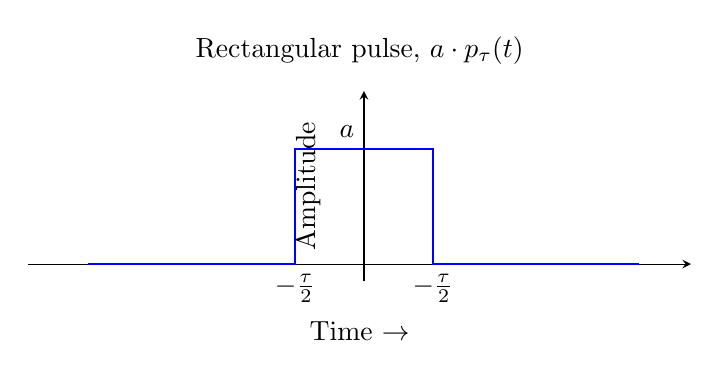
\begin{tikzpicture}
    	\begin{axis}[
    	width=10cm,
    	height=4cm,
    	x axis line style={-stealth},
    	y axis line style={-stealth},
    	title={Rectangular pulse, $a \cdot p_\tau(t)$},
    	xtick={-1,1},
    	xticklabels={$-\frac{\tau}{2}$,$-\frac{\tau}{2}$},
    	ymax = 1.5,xmax=4.75,
    	axis lines*=center,
    	ytick={1.15},
    	yticklabels={$a$},
    	ytick style={draw=none},
    	xlabel={Time $\rightarrow$},
    	ylabel={Amplitude}
    	]
    	\addplot+[thick,mark=none,const plot]
    	coordinates
    	{(-4,0) (-1,0) (-1,1) (1,1) (1,0) (4,0)};
    	\end{axis}
    	\end{tikzpicture}
    \end{figure}
    
    We know that the Fourier transform of some signal, $x(t)$, is given by:
    
    \begin{align*}
	    \mathscr{F}\{x(t)\} = X(\omega) = \int_{-\infty}^{\infty}x(t)e^{-j \omega t}dt
    \end{align*}
    
    Hence, for the rectangular pulse, we get that:
    
    \begin{align*}
	    \mathscr{F}\{a \cdot p_\tau (t)\} 	&= \int_{-\infty}^{\infty}a \cdot p_\tau (t)e^{-j \omega t}dt\\
										    &= a \int_{-\frac{\tau}{2}}^{\frac{\tau}{2}} p_\tau (t)e^{-j \omega t}dt\\
										    &= a \int_{-\frac{\tau}{2}}^{\frac{\tau}{2}} e^{-j \omega t}dt\\
										    &= a \bigg[ -\frac{1}{j \omega} e^{-j \omega t}\bigg]^{\frac{\tau}{2}}_{-\frac{\tau}{2}}\\
										    &= -\frac{a}{j \omega}\big( e^{-j \omega \frac{\tau}{2}} - e^{j \omega \frac{\tau}{2}} \big)\\
										    &= -\frac{a}{j \omega}\big( \cos(\frac{\omega \tau}{2}) - j\sin(\frac{\omega \tau}{2}) - \cos(\frac{\omega \tau}{2}) - j\sin(\frac{\omega \tau}{2}) \big)\\
										    &= \frac{2a}{\omega}\sin(\frac{\omega \tau}{2})
    \end{align*}
	
	Now, given that:
	
	\begin{align*}
		\sinc(A \omega) = \frac{ \sin(A \pi \omega)}{A \pi \omega}
	\end{align*}
	
	Hence, we can see that:
	
	\begin{align*}
		\sin(A \omega) &= \sin(\frac{\omega \tau}{2})\\
		\therefore A &= \frac{\tau}{2 \pi}
	\end{align*}
	
	Hence, we can write our transform in terms of the $\sinc$ function:
	
	\begin{align*}
		\mathscr{F}\{a \cdot p_\tau (t)\} 	&= 2a \cdot \frac{\sin(A \pi \omega)}{A \pi \omega} \cdot A \pi\\
											&= 2a \cdot A \pi \cdot \sinc(A \omega)\\
											&= 2a \cdot \frac{\tau}{2 \pi} \pi \sinc(\frac{\tau \omega}{2 \pi})\\
											&= a \tau \sinc(\frac{\tau \omega}{2 \pi})
	\end{align*}
	
	Finally, suppose that we had a pulse rectangle $p_2(t)$ with an amplitude of 1, then the Fourier transform would be:
	
	\begin{align*}
		\mathscr{F}\{p_2(t)\} 	&= 1 \cdot 2 \cdot \sinc(\frac{2 \omega}{2 \pi})\\
								&= 2 \cdot \sinc(\frac{\omega}{\pi})
	\end{align*}
	
\end{homeworkProblem}

\pagebreak

%%%%%%%%%%%%%%%%%%%%%%%%%%%%%%%%%%%%%%%%%%%%%%%%%%%%%%%%%%%%%%%%%%%%%%%%%%%%%%%%%%%%%%%%%%%%%%%%%%%%%%%%%%%%%%%%%%%%%%
% Question 4
%%%%%%%%%%%%%%%%%%%%%%%%%%%%%%%%%%%%%%%%%%%%%%%%%%%%%%%%%%%%%%%%%%%%%%%%%%%%%%%%%%%%%%%%%%%%%%%%%%%%%%%%%%%%%%%%%%%%%%

\begin{homeworkProblem}
    
    \textbf{Fourier Transforms}\\
    
    \textsc{Question a}\\
    
    Consider the following signal $v(t)$:
    \begin{figure}[h]
    	\centering
    	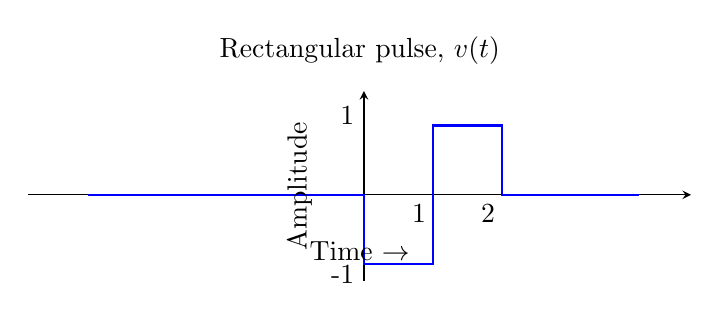
\begin{tikzpicture}
    	\begin{axis}[
    	width=10cm,
    	height=4cm,
    	x axis line style={-stealth},
    	y axis line style={-stealth},
    	title={Rectangular pulse, $v(t)$},
    	xtick={0.8,1.8},
    	xticklabels={1,2},
    	xtick style={draw=none},
    	ymax = 1.5,xmax=4.75,
    	axis lines*=center,
    	ytick={-1.15,1.15},
    	yticklabels={-1,1},
    	ytick style={draw=none},
    	xlabel={Time $\rightarrow$},
    	ylabel={Amplitude}
    	]
    	\addplot+[thick,mark=none,const plot]
    	coordinates
    	{(-4,0) (0,0) (0,-1) (1,-1) (1,1) (2,1) (2,0) (4,0)};
    	\end{axis}
    	\end{tikzpicture}
    \end{figure}
    
    This pulse can be written as follows:
    
    \begin{align*}
	    v(t) = -p_1(t - \sfrac{1}{2}) + p_1(t - \sfrac{3}{2})
    \end{align*}
    
    The Fourier transform of $v(t)$, using standard transforms we get:
    
    \begin{align*}
	    \mathscr{F}\{v(t)\} = -1 \cdot \sinc(\frac{\omega}{2 \pi})e^{-j \omega \sfrac{1}{2}} + \sinc(\frac{\omega}{2 \pi})e^{-j \omega \sfrac{3}{2}}
    \end{align*}
    
    \vspace{5mm}
    
    \textsc{Question b}\\
    
    Consider the following signal $v(t)$:
    \begin{figure}[h]
    	\centering
    	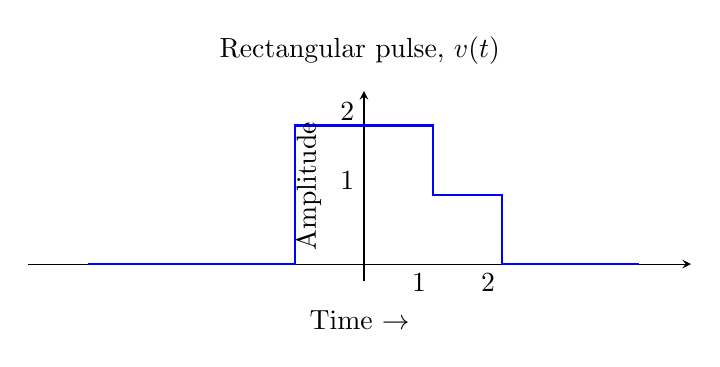
\begin{tikzpicture}
    	\begin{axis}[
    	width=10cm,
    	height=4cm,
    	x axis line style={-stealth},
    	y axis line style={-stealth},
    	title={Rectangular pulse, $v(t)$},
    	xtick={0.8,1.8},
    	xticklabels={1,2},
    	xtick style={draw=none},
    	ymax = 2.5,xmax=4.75,
    	axis lines*=center,
    	ytick={1.2,2.2},
    	yticklabels={1,2},
    	ytick style={draw=none},
    	xlabel={Time $\rightarrow$},
    	ylabel={Amplitude}
    	]
    	\addplot+[thick,mark=none,const plot]
    	coordinates
    	{(-4,0) (-1,0) (-1,2) (1,2) (1,1) (2,1) (2,0) (4,0)};
    	\end{axis}
    	\end{tikzpicture}
    \end{figure}
    
    This pulse can be written as follows:
    
    \begin{align*}
    v(t) = p_3(t - \sfrac{1}{2}) + p_2(t)
    \end{align*}
    
    The Fourier transform of $v(t)$, using standard transforms we get:
    
    \begin{align*}
    \mathscr{F}\{v(t)\} = -1 \cdot \sinc(\frac{\omega}{2 \pi})e^{-j \omega \sfrac{1}{2}} + \sinc(\frac{\omega}{2 \pi})e^{-j \omega \sfrac{3}{2}}
    \end{align*}
    
\end{homeworkProblem}

\pagebreak

%%%%%%%%%%%%%%%%%%%%%%%%%%%%%%%%%%%%%%%%%%%%%%%%%%%%%%%%%%%%%%%%%%%%%%%%%%%%%%%%%%%%%%%%%%%%%%%%%%%%%%%%%%%%%%%%%%%%%%
% Question 5
%%%%%%%%%%%%%%%%%%%%%%%%%%%%%%%%%%%%%%%%%%%%%%%%%%%%%%%%%%%%%%%%%%%%%%%%%%%%%%%%%%%%%%%%%%%%%%%%%%%%%%%%%%%%%%%%%%%%%%

\begin{homeworkProblem}
	
    Consider the signal $x(t) \longleftrightarrow X(\omega)$. The plot of $X(\omega)$ is shown below.
    
    \begin{figure}[h]
    	\centering
    	\begin{tikzpicture}
    	\begin{axis}[
    	width=10cm,
    	height=4cm,
    	x axis line style={-stealth},
    	y axis line style={-stealth},
    	title={$X(\omega)$},
    	xtick={-2,2},
    	xticklabels={-2,2},
    	xtick style={draw=none},
    	ymax = 1.5,
    	axis lines*=center,
    	ytick={1.2},
    	yticklabels={$A$},
    	ytick style={draw=none},
    	xlabel={Frequency ($\omega$)}
    	]
    	\addplot+[thick,mark=none]
    	coordinates
    	{(-4,0) (-2,0) (0,1) (2,0) (4,0)};
    	\end{axis}
    	\end{tikzpicture}
    \end{figure}
    
    Suppose a new signal, $v(t)$, was composed by multiplying $x(t)$ by $\cos(5t)$. The Fourier transform would be:
    
    \begin{align*}
	    x(t) \cdot \cos(5t) \longleftrightarrow \frac{1}{2} \cdot \bigg[X(\omega +5) + X(\omega - 5)\bigg].
    \end{align*}
    
    The plot of the Fourier transform of $v(t)$, $V(\omega)$, is shown below.
    
    \begin{figure}[h]
    	\centering
    	\begin{tikzpicture}
    	\begin{axis}[
    	width=10cm,
    	height=4cm,
    	x axis line style={-stealth},
    	y axis line style={-stealth},
    	title={$V(\omega)$},
    	xtick={-7,-3,3,7},
    	xticklabels={-7,-3,3,7},
    	xtick style={draw=none},
    	ymax = 1.5,
    	axis lines*=center,
    	ytick={0.7},
    	yticklabels={$\frac{A}{2}$},
    	ytick style={draw=none},
    	xlabel={Frequency ($\omega$)}
    	]
    	\addplot+[thick,mark=none]
    	coordinates
    	{(-9,0) (-7,0) (-5,0.5) (-3,0) (3,0) (5,0.5) (7,0) (9,0)};
    	\end{axis}
    	\end{tikzpicture}
    \end{figure}
    
    Suppose now that the signal $v(t)$ was passed through some filter $H_1(\omega)$, such that:
    
    \[
    H_1(\omega) =
    \begin{cases} 
    \hfill 2 \hfill & \text{ if $3 \leq |\omega| \leq 5$} \\
    \hfill 0 \hfill & \text{ all other $\omega$} \\
    \end{cases}
    \]
    
    If $W(\omega) = H_1(\omega)V(\omega)$, then a plot of $W(\omega)$ is shown below:
    
    \begin{figure}[h]
    	\centering
    	\begin{tikzpicture}
    	\begin{axis}[
    	width=10cm,
    	height=4cm,
    	x axis line style={-stealth},
    	y axis line style={-stealth},
    	title={$W(\omega)$},
    	xtick={3,5},
    	xticklabels={3,5},
    	xtick style={draw=none},
    	ymax = 1.5,
    	axis lines*=center,
    	ytick={1.2},
    	yticklabels={$A$},
    	ytick style={draw=none},
    	xlabel={Frequency ($\omega$)}
    	]
    	\addplot+[thick,mark=none]
    	coordinates
    	{(-9,0) (3,0) (5,1) (5,0) (9,0)};
    	\end{axis}
    	\end{tikzpicture}
    \end{figure}
    
    \newpage
    
    Now, if $w(t) \longleftrightarrow W(\omega)$, then we can create some new signal, $r(t)$, such that $r(t) = w(t) \cdot \cos(3t)$. The new signal has the following transform:
    
    \begin{align*}
	    w(t) \cdot \cos(3t) \longleftrightarrow \frac{1}{2}\bigg[W(\omega + 3) + W(\omega - 3)\bigg]
    \end{align*}
    
    The plot of the Fourier transform of $r(t)$, $R(\omega)$, is shown below:
    
    \begin{figure}[h]
    	\centering
    	\begin{tikzpicture}
    	\begin{axis}[
    	width=10cm,
    	height=4cm,
    	x axis line style={-stealth},
    	y axis line style={-stealth},
    	title={$R(\omega)$},
    	xtick={2,6,8},
    	xticklabels={2,6,8},
    	xtick style={draw=none},
    	ymax = 1.5,
    	axis lines*=center,
    	ytick={0.7},
    	yticklabels={$\frac{A}{2}$},
    	ytick style={draw=none},
    	xlabel={Frequency ($\omega$)}
    	]
    	\addplot+[thick,mark=none]
    	coordinates
    	{(-9,0) (0,0) (2,0.5) (2,0) (6,0) (8,0.5) (8,0) (9,0)};
    	\end{axis}
    	\end{tikzpicture}
    \end{figure}
    
    Finally, suppose that $r(t)$ was passed through some filter $H_2(\omega)$, such that:
    
    \[
    H_2(\omega) =
    \begin{cases} 
    \hfill 2 \hfill & \text{ if $|\omega| \leq 3$} \\
    \hfill 0 \hfill & \text{ all other $\omega$} \\
    \end{cases}
    \]
    
    If $Y(\omega) = H_2(\omega)R(\omega)$, then a plot of $Y(\omega)$ is shown below:
    
    \begin{figure}[h]
    	\centering
    	\begin{tikzpicture}
    	\begin{axis}[
    	width=10cm,
    	height=4cm,
    	x axis line style={-stealth},
    	y axis line style={-stealth},
    	title={$Y(\omega)$},
    	xtick={2},
    	xticklabels={2},
    	xtick style={draw=none},
    	ymax = 1.5,
    	axis lines*=center,
    	ytick={1.2},
    	yticklabels={$A$},
    	ytick style={draw=none},
    	xlabel={Frequency ($\omega$)}
    	]
    	\addplot+[thick,mark=none]
    	coordinates
    	{(-9,0) (0,0) (2,1) (2,0) (9,0)};
    	\end{axis}
    	\end{tikzpicture}
    \end{figure}
    
\end{homeworkProblem}

\end{document}
